\documentclass[
	% -- opções da classe memoir --
	article,			% indica que é um artigo acadêmico
	12pt,				% tamanho da fonte
	oneside,			% para impressão apenas no recto. Oposto a twoside
	a4paper,			% tamanho do papel.
	% -- opções da classe abntex2 --
	%chapter=TITLE,		% títulos de capítulos convertidos em letras maiúsculas
	%section=TITLE,		% títulos de seções convertidos em letras maiúsculas
	%subsection=TITLE,	% títulos de subseções convertidos em letras maiúsculas
	%subsubsection=TITLE % títulos de subsubseções convertidos em letras maiúsculas
	% -- opções do pacote babel --
	english,			% idioma adicional para hifenização
	brazil,				% o último idioma é o principal do documento
	sumario=tradicional
	]{abntex2}


% ---
% PACOTES
% ---

\usepackage{lmodern}			% Usa a fonte Latin Modern
\usepackage[T1]{fontenc}		% Selecao de codigos de fonte.
\usepackage[utf8]{inputenc}		% Codificacao do documento (conversão automática dos acentos)
\usepackage{indentfirst}		% Indenta o primeiro parágrafo de cada seção.
\usepackage{float}
\usepackage{nomencl} 			% Lista de simbolos
\usepackage{color}				% Controle das cores
\usepackage{graphicx}			% Inclusão de gráficos
\usepackage{microtype} 			% para melhorias de justificação
% ---

% ---
% Pacotes de citações
% ---
\usepackage[brazilian,hyperpageref]{backref}	 % Paginas com as citações na bibl
\usepackage[alf]{abntex2cite}	% Citações padrão ABNT
% ---

% ---
%Caminho das imagens
\graphicspath{ {images/} }
% ---

% ---
% Configurações do pacote backref
% Usado sem a opção hyperpageref de backref
\renewcommand{\backrefpagesname}{Citado na(s) página(s):~}
% Texto padrão antes do número das páginas
\renewcommand{\backref}{}
% Define os textos da citação
\renewcommand*{\backrefalt}[4]{
	\ifcase #1 %
		Nenhuma citação no texto.%
	\or
		Citado na página #2.%
	\else
		Citado #1 vezes nas páginas #2.%
	\fi}%
% ---

% ---
% Informações de dados para CAPA e FOLHA DE ROSTO
% ---
\titulo{Análise de vulnerabilidade e segurança de redes sem fio comerciais}
\autor{
Angelo Rodrigo Ribeiro da Silva\thanks{angelorodriigo.rs@gmail.com} Jaíne da Silva Santos\thanks{jaine.ssilva1@gmail.com}
\\Jonatas Rosa da Silva Bonventi\thanks{jonatasbvt@yahoo.com}
}
\local{Boituva}
\data{2017}

% Configurações de aparência do PDF final

% alterando o aspecto da cor azul
\definecolor{blue}{RGB}{41,5,195}

% informações do PDF
\makeatletter
\hypersetup{
     	%pagebackref=true,
		pdftitle={\@title},
		pdfauthor={\@author},
    	pdfsubject={Análise de vulnerabilidade de redes utilizando técnicas de WarDriving},
	    pdfcreator={LaTeX with abnTeX2},
		pdfkeywords={wardriving}{Wifi}{segurança da informação}{ifsp},
		colorlinks=true,       		% false: boxed links; true: colored links
    	linkcolor=blue,          	% color of internal links
    	citecolor=blue,        		% color of links to bibliography
    	filecolor=magenta,      		% color of file links
		urlcolor=blue,
		bookmarksdepth=4
}
\makeatother

% compila o indice
\makeindex

% Margens segundo abnt
\setlrmarginsandblock{3cm}{3cm}{*}
\setulmarginsandblock{3cm}{3cm}{*}
\checkandfixthelayout

% ---
% Espaçamentos entre linhas e parágrafos
% ---

% O tamanho do parágrafo é dado por:
\setlength{\parindent}{1.3cm}

% Controle do espaçamento entre um parágrafo e outro:
\setlength{\parskip}{0.2cm}  % tente também \onelineskip

% Espaçamento simples
\SingleSpacing

% Início do documento
\begin{document}

% Seleciona o idioma do documento (conforme pacotes do babel)
\selectlanguage{brazil}

% Retira espaço extra obsoleto entre as frases.
\frenchspacing

% ELEMENTOS PRÉ-TEXTUAIS
% página de titulo
\maketitle

% resumo em português
\begin{resumoumacoluna}
Com a crescente demanda de dispositivos móveis conectados à internet, como celulares, tablets e notebooks, o uso de redes sem fio tornou-se algo bastante presente em nosso dia-a-dia. Seja em ambientes corporativos ou domésticos, a popularização deu-se também pela facilidade e liberdade que a tecnologia wireless fornece, e recentemente invadiu outros dispositivos pelo fenômeno chamado Internet das Coisas (IoT), como eletrodomésticos, carros e roupas.\\

Entretanto, a maioria dessas redes não é protegida de forma adequada, tornando-se constantemente “portas de entrada” para hackers sequestrarem informações de usuários ou sabotarem sistemas que gerarão grandes prejuízos.\\

 \vspace{\onelineskip}

 \noindent
 \textbf{Palavras-chave}: Wardriving. Segurança da informação.
\end{resumoumacoluna}

% ELEMENTOS TEXTUAIS
\textual

% Introdução
\section*{Introdução}
\addcontentsline{toc}{section}{Introdução}
\nocite{varredura-ibirama}
\nocite{analise-vulnerabilidade}

Segundo \cite[p. 67]{redes-tanenbaum} "Quase na mesma época em que surgir am os notebooks, muitas pessoas sonhavam com o dia em que entrariam em um escritório e magicamente seu notebook se conectaria à Internet.", e logicamente, veio logo após a necessidade de proteger essas redes através de criptografia e outras técnicas de segurança.\\

E também, com a melhora de segurança das redes, surgiram pessoas interessadas em quebrar essas redes, seja por interesse financeiro, corporativo ou mesmo pelo triunfo de se atingir um objetivo utilizando técnicas de quebra, prática muito comum nas comunidades de hackers.

\section{Wardriving}

Ao contrário do que se acredita, Wardriving não é uma técnica ilegal ou invasiva, visto que não são obtidas informações que estão encapsuladas na mensagem trocada entre dispositivos sem autorização das partes afetadas, ou seja, não existe quebra de sigilo. Existindo muitas formas de executar os testes, muitas vezes são utilizadas ferramentas que são comuns aos hackers para invasão de redes, e por esse motivo os conceitos são associados de forma errônea.\\

A definição básica de wardriving consiste no testador mover-se em uma área específica, mapeando a população de pontos de acesso sem fio existentes. Os resultados obtidos são utilizados para levantar vulnerabilidades existentes por meio das informações que os equipamentos dispõem, como se é utilizado criptografia (e de qual tipo). Sendo uma prática relativamente simples, pode ser realizada por hobistas ou profissionais que futuramente utilizarão as informações obtidas para conduzir testes de penetração, por exemplo.\\

Também é relevante mencionar que com a crescente preocupação em segurança de informação como forma de prevenir incidentes, a procura por profissionais capacitados a identificar e analisar vulnerabilidades também aumentou exponencialmente.

\section{Protocolas de segurança em redes sem fio}

Primeiramente, é necessário compreender o funcionamento básico das formas mais comuns de proteger redes sem fio, bem como seu posicionamento no contexto tecnológico atual. A maioria dos roteadores modernos possuem recursos para configuração fácil pelo próprio usuário, e a mais antiga que foi padrão de mercado por bastante tempo é a chamada WEP.\\

Esse modelo foi adotado como padrão de segurança em setembro de 1999 e desde então tem sido o protocolo mais difundido para redes sem fio, e em sua forma mais comum tratava-se de uma implementação com chave de 128 bits para encriptação dos dados. A partir de 2001, uma série de exploits foram criados aproveitando inúmeras vulnerabilidades que tecnologia possui, e mesmo sendo melhor do que manter uma rede sem proteção alguma, não é recomendado atualmente.\\

Como prova disso, o FBI (US Federal Bureau of Investigation) forneceu em 2005 uma demonstração pública onde foi realizada a quebra de segurança em pouco minutos, utilizando uma ferramenta gratuita.\\

Posteriormente, surgiram novos padrões como WPA (Wi-Fi Protected Access) em 2003 utilizando chave PSK e de 256 bits e WPA2 em 2006 com uma série de melhorias como o uso mandatório de algoritmos AES. Atualmente, aparelhos mais completos no mercado permitem a combinação de algumas tecnologias de autenticação e métodos de criptografia para sanar algumas vulnerabilidades ainda existentes. É possível verificar abaixo uma relação com as tecnologias mais seguras disponíveis para o público geral em ordem decrescente:\\

\begin{enumerate}
\item{WPA + AES}
\item{WPA + AES}
\item{WPA + TKIP/AES (TKIP atua como método de contingência)}
\item{WPA + TKIP}
\item{WEP}
\item{Rede aberta (sem protocolo de segurança)}
\end{enumerate}

Os critérios acima serão utilizados como referência para estudo do ambiente selecionado, cujo índice de vulnerabilidade poderá variar de acordo com outras condições como existência de logins, autenticação de 2 fatores, redes ocultas, entre outros.\\

\section{Análise de vulnerabilidade e tentativa de quebra de senhas}

Buscando analisar a vulnerabilidade de redes wifi de estabelecimentos, fomos a um shopping em Sorocaba avaliar as redes através de wardriving e depois tentarmos quebrar redes.

\subsection{Objetivos}

O nosso objetivo é verificar se os grandes estabelecimentos se preocupam com segurança de redes, visto que milhares de usuários acessam a rede todos os dias.

\subsection{Ferramentas utilizadas}

\subsubsection{Kismet}

Nós utilizamos o Kismet para realizar wardriving e capturar estátisticas e pacotes das redes wifi e salvar essas informações utilizando gps, para podermos analizar após.

\subsubsection{Wireshark}

Para as redes abertas, decidimos capturar os pacotes enviados e recebidos de toda a rede utilizando wireshark.

\subsubsection{Aircrack}

Para as redes fechadas, com a captura de pacotes, fizemos então handshake, e após, tentativas de quebra utilizando wordlists de 13.2 gb com 1.2 bilhão de senhas.

\subsection{Resultados da análise de redes}

\subsubsection{Captura de pacotes}

Conseguimos capturar através do Kismet 37 redes sem fio válidas (com conexão), das quais 22 eram redes abertas que foram analisadas utilizando sniffing e 15 eram redes privadas.

\begin{figure}[H]
	\centering
	\caption{Gráfico das seguranças de redes sem fio utilizadas.}
	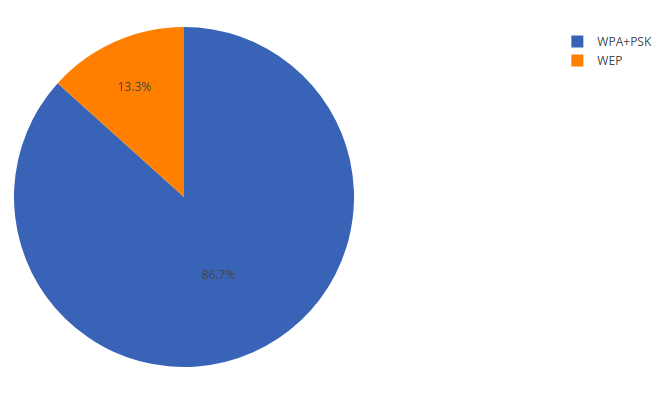
\includegraphics[scale=0.7]{graficopie-seguranca-redes}
\end{figure}

Como podemos ver acima, a maior parte das redes wifi privadas utilizam a criptografia de rede WPA2-PSK, porém ainda temos redes que utizam protocolo WEP, que é muito inseguro e fácil de ser quebrado.

\subsubsection{Cracking de senhas}

Após feita a captura dos pacotes, capturamos os handshakes utilizando o comando aireplay-ng do pacote aircrack.\\

\subsubsubsection{WPA-PSK}

Para redes WPA-PSK, utilizamos um arquivo word-list contendo 1.2 bilhão de senhas mais utilizadas em redes sem fio, utilizando o aircrack-ng.\\

Das redes WPA-PSK analisadas, nenhuma foi quebrada, mesmo após utilizar toda a lista.\\

\subsubsubsection{WEP}

Já as duas redes WEP foram quebradas em pouco tempo utilizando o aircrack-ng com a flag 1 ativada, que decripta handshakes de redes WEP.

\subsubsection{Sniffing}

Nas redes abertas, foram feitas tentativas de sniffing nos pacotes que estavam sendo transmitidos utilizando wireshark.

\begin{figure}[H]
	\centering
	\caption{Sniffing de rede sem fio utilizando wireshark.}
	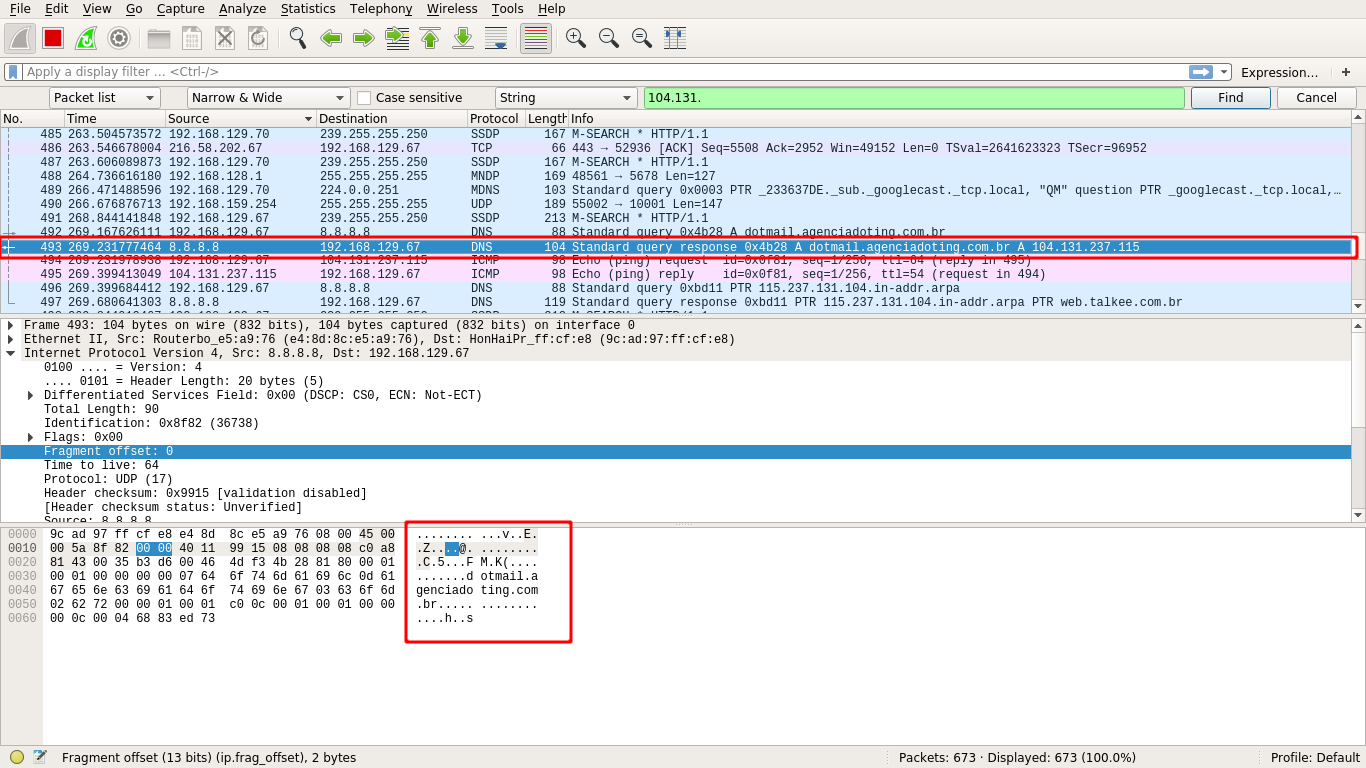
\includegraphics[scale=0.32]{captura-wireshark-1}
\end{figure}

Na figura acima, vemos em destaque uma requisição do tipo GET capturada que foi feita por nós, vemos aqui que as requisições não são criptografadas pelo roteador.\\

Indo além, uma pessoa mal intencionada poderia também capturar informações de uma requisição do tipo POST, para posteriormente descriptografar as informações passadas pelos headers.\\

% Finaliza a parte no bookmark do PDF, para que se inicie o bookmark na raiz
\bookmarksetup{startatroot}

% Conclusão
\section*{Considerações finais}
\addcontentsline{toc}{section}{Considerações finais}

Vimos que mesmo hoje em dia, existem redes sem fio comerciais(estabelecimentos etc), que utilizam protocolos de segurança fracos, uma indicação é procurar configurar no roteador um protocolo de segurança, e para grandes ambientes, criptografar as requisições, ou seja, tudo que entra e sai da rede.

% Elementos pós textuais
\postextual

% Titulo e resumo em outro idioma
\titulo{Vulnerability Analysis of Commercial Wireless Networks}
\emptythanks
\maketitle

\renewcommand{\resumoname}{Abstract}
\begin{resumoumacoluna}
 \begin{otherlanguage*}{english}

With the growing-up demand of mobile devices, as smartphones, tablets and laptops, the use of wireless networks became highly present in our routine. Whether it’s in corporative or domestic environments, the popularization happened also due facility and freedom wireless networks provide, and recently, invaded another devices due Internet of Things (IoT) phenomena such as home appliances, cars and clothes.\\

However, most of these networks aren’t properly protected, turning them into “entry doors” for hackers hijacking information from users or sabotage systems which will cause massive losses.

   \vspace{\onelineskip}

 \noindent
 \textbf{Keywords}: Wardriving. Information Security.
 \end{otherlanguage*}
\end{resumoumacoluna}

% Referências bibliográficas
\bibliography{wardriving}

\end{document}
\grid
